\documentclass[10pt,letterpaper]{article}
\usepackage[top=0.85in,left=2.75in,footskip=0.75in,marginparwidth=2in]{geometry}

% use Unicode characters - try changing the option if you run into troubles with special characters (e.g. umlauts)
\usepackage[utf8]{inputenc}

% clean citations
\usepackage{cite}

% hyperref makes references clicky. use \url{www.example.com} or \href{www.example.com}{description} to add a clicky url
\usepackage{nameref,hyperref}

% line numbers
\usepackage[right]{lineno}

% improves typesetting in LaTeX
\usepackage{microtype}
\DisableLigatures[f]{encoding = *, family = * }

% text layout - change as needed
\raggedright
\setlength{\parindent}{0.5cm}
\textwidth 5.25in 
\textheight 8.75in

% Remove % for double line spacing
%\usepackage{setspace} 
%\doublespacing

% use adjustwidth environment to exceed text width (see examples in text)
\usepackage{changepage}

% adjust caption style
\usepackage[aboveskip=1pt,labelfont=bf,labelsep=period,singlelinecheck=off]{caption}

% remove brackets from references
\makeatletter
\renewcommand{\@biblabel}[1]{\quad#1.}
\makeatother

% headrule, footrule and page numbers
\usepackage{lastpage,fancyhdr,graphicx}
\usepackage{epstopdf}
\pagestyle{myheadings}
\pagestyle{fancy}
\fancyhf{}
\rfoot{\thepage/\pageref{LastPage}}
\renewcommand{\footrule}{\hrule height 2pt \vspace{2mm}}
\fancyheadoffset[L]{2.25in}
\fancyfootoffset[L]{2.25in}

% use \textcolor{color}{text} for colored text (e.g. highlight to-do areas)
\usepackage{color}

% define custom colors (this one is for figure captions)
\definecolor{Gray}{gray}{.25}

% this is required to include graphics
\usepackage{graphicx}

% use if you want to put caption to the side of the figure - see example in text
\usepackage{sidecap}

% use for have text wrap around figures
\usepackage{wrapfig}
\usepackage[pscoord]{eso-pic}
\usepackage[fulladjust]{marginnote}
\reversemarginpar

% document begins here
\begin{document}
\vspace*{0.35in}

% title goes here:
\begin{flushleft}
{\Large
\textbf\newline{Global-scale microbial ecology of functional anchors with TreeSAPP}
}
\newline
% authors go here:
\\
Author 1\textsuperscript{1},
Author 2\textsuperscript{2},
Author 3\textsuperscript{1},
Author 4\textsuperscript{1},
Author 5\textsuperscript{2},
Author 6\textsuperscript{2},
Author 7\textsuperscript{1,*}
\\
\bigskip
\bf{1} Affiliation A
\\
\bf{2} Affiliation B
\\
\bigskip
* shallam@mail.ubc.ca

\end{flushleft}

\section*{Abstract}
We present an updated version of TreeSAPP with an expanded capacity for facilitating microbial ecological analyses using functional marker genes. TreeSAPP builds off the foundations built by phylogenetic placement tools to enable users to rapidly screen metagenomic datasets for genes of interest, compare them within an evolutionary framework, and conduct classical microbial ecology analyses. We end by touching on best practices for gene-centric analyses.

% now start line numbers
\linenumbers

% the * after section prevents numbering
\section*{Introduction}
	Microbial ecology has been dominated by studies harnessing a limited set of universal single copy marker genes such as the 16S rRNA gene. Only recently have genome-wide studies been made available and supported by a robust and dependable network of bioinformatic tools. However, a perennial problem with genome-centric metagenomics with metagenome-assembled genomes (MAGs) and single-cell amplified genomes (SAGs) is the lack of community representation. In most cases, SAGs are prohibitively expensive to generate sufficient coverage across the community, even in light of new methods for functionally screening single cells to guide sequencing efforts. With short-reads alone, the majority of scaffolds assembled from a metagenomic dataset are too short to be binned and therefore the majority of a microbial community is omitted from its corresponding MAG dataset. Therefore, an alternative approach is required to comprehensively sample and analyze the functional capacity of microbial communities.
	Gene-centric analyses, using both amplified and unprocessed sequence information, have long had a place in a microbial ecologist's tool box. We propose that studies focusing on functional guilds turn to TreeSAPP for facilitating analyses into guild presence and diversity of microbiomes.

\textbf{Key points}
\begin{enumerate}
\item Single file reference packages for easier portability and thus reproducibility; guide to the publicly-available community resource.
\item Recommendations for using merged paired-end reads or assemblies
\item Replaced RAxML with EPA-NG and RAxML-NG leading to better computational performance (RAM and time requirements compared to older version)
\item Phylogenetic clustering
\item Compare accumulated likelihood weight ratio (LWR) to maximum LWR with linear model for taxonomic assignment
\item Evolutionary distance as an indicator to update
\item Comparison to PhyloMagnet and GraftM?
\item Why not EggNOG-mapper or other tools?
\end{enumerate}

\section*{Materials and Methods}

\paragraph{}

\paragraph{Taxonomic classification of ORFs from raw, merged, and assembled reads}

Simulated metagenome reads and contigs were obtained from the first Critical Assessment of Metagenome Interpretation (CAMI) challenge\cite{Sczyrba2017}. The reads were merged using BBMerge version 38.89 with default parameters and the 'gold\_standard\_high\_single' metagenome assembly was used without modification \cite{Bushnell2017}. TreeSAPP version \textbf{X.YY.Z} was used to classify sequences from the three datasets using nineteen reference packages that were commonly found in the metagenome (supplementary table 2). Briefly, Prodigal (version 2.6.3) predicted ORFs, homologous sequences were detected by hmmsearch then aligned to reference sequences with hmmalign (version 3.3.2) before phylogenetic placement using EPA-NG (version 0.3.8) \cite{Hyatt2012,Eddy1998a,Barbera2018}. The minimum profile HMM coverage was set to 10\% to retain enough ORFs from the unmerged reads for the comparative analysis. This would lead to more false positive classifications, especially among the reference packages involved in respiration.

\paragraph{Phylogenetic clustering}

Determining the breadth of diversity and functional redundancy is critical to understanding the biogeochemistry of an environmental system. We sought to find a method that allows for accurate clustering of metagenomic ORFs, which are often truncated. Being incomplete sequences, this could be an issue for both traditional pairwise clustering approaches that perform best with full-length sequences and phylogenetic clustering methods that partition the leaf nodes based on an evolutionary distance threshold. To address this, we compared these two methods to one that leverages the phylogenetic placements resulting from taxonomic classification by partitioning the internal and leaf edges. The primary drawback of this approach is disregarding the pendant length distance of a query placement, which may be large enough to prevent a sequence from belonging in a phylogenetic cluster. Regardless, our naive approach assumes this is a rare case and compares favourably (Figure 1A). 
In this comparison we evaluated the three methods on their ability to ensure queries from related organisms belonged to the same cluster, unrelated organisms belonged to different clusters and instances where related sequences belonged to different clusters was mitigated.
We chose eighteen genomes (eight Bacteria and ten Archaea; Supplementary Table 1) with three functional (McrA, NifH and SoxB) and two housekeeping (RpoB and Ribosomal protein L32) reference packages. Three different thresholds were used to approximate taxonomic species-, family- and class-resolved clusters. Genomes were 

\marginpar{
\vspace{.7cm} % adjust vertical position relative to text with \vspace{} - note that you can enter negative numbers to move margin caption up
\color{Gray} % this gives caption a grey color to set it apart from text body
\textbf{Figure \ref{fig1}. Example of a margin caption.} % note that \ref{fig1} refers to the corresponding wrapfigure
Setting up your figure + caption like this looks fancy and does not disrupt the flow of the text. But it requires more manual adjustments (position, spacing, labeling) compared to using standard \LaTeX figure environments.
}

\begin{wrapfigure}[19]{l}{75mm}
% the number in [] of wrapfigure is optional and gives the number of text lines that should be wrapped around the text. Adjust according to your figures height
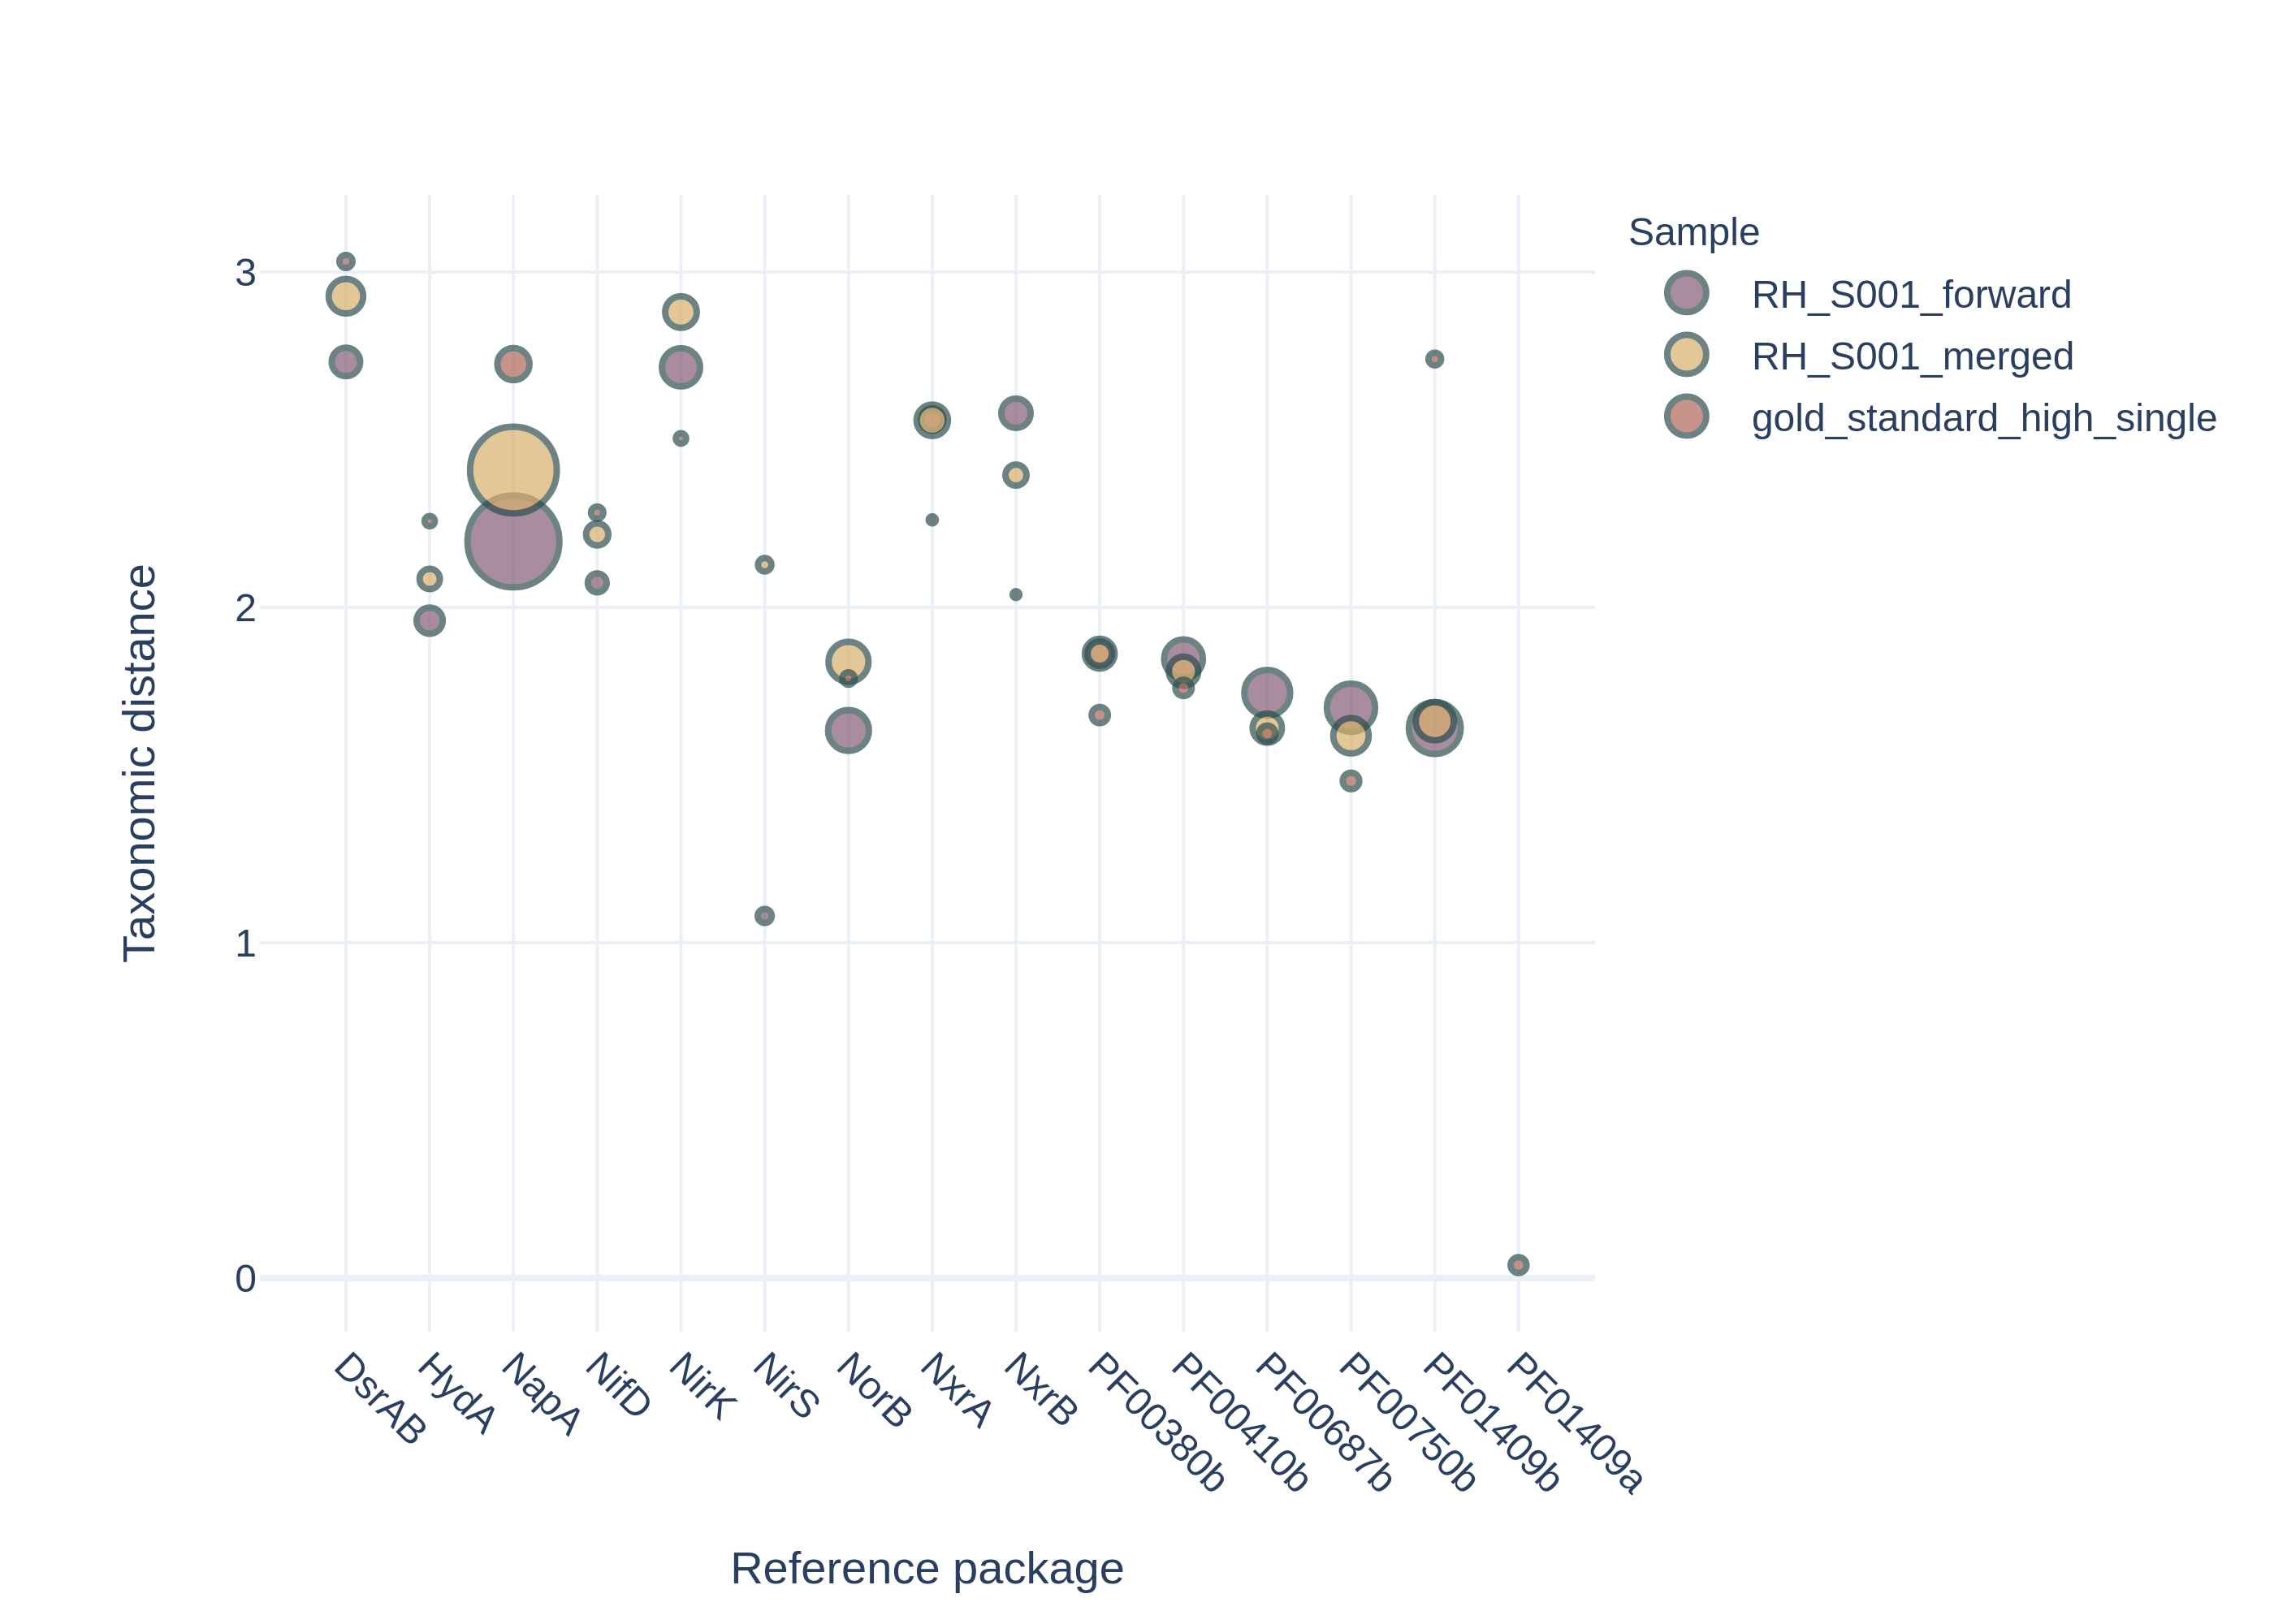
\includegraphics[width=75mm]{manuscript/figures/tax_dist_bubbles.png}
\captionsetup{labelformat=empty} % makes sure dummy caption is blank
\caption{} % add dummy caption - otherwise \label won't work and figure numbering will not count up
\label{fig1} % use \ref{fig1} to reference to this figure
\end{wrapfigure} % avoid blank space here
the \verb!marginnote! environment. Please note that in this case the figure (\verb!wrapfigure!) and the figure caption (\verb!marginpar!) have to be separated as you can tell from the code. The \verb!wrapfigure! environment can be a bit tricky when it comes to text formatting. Thus some general hints: (a) try to avoid line breaks in the code as this may result in weird formatting around the figure, (b) the figure should not span multiple headlines (sections) and (c) if you encounter problems with the line break right after the \verb!wrapfigure! try using \verb!\mbox{}! to prevent premature line breaks (\mbox{see example in code}). As stated in the figure caption, setting up figures this way requires a bit more manual adjustments but it makes figures blend in nicely without interrupting flow of text.


\section*{Results}
\subsection*{Merged reads balance richness and accuracy best}
The number of predicted ORFs and average ORF lengths were 46,760,971 and 46.9, 21,180,042 and 71.3, and 2,640,031 and 313.9 for the forward reads, merged reads and the contigs, respectively (supplementary table 1). The most ORFs were classified from the merged reads (34918), followed by the forward reads (24765) and the contigs (12591).
Taxonomic classification accuracy was compared between the three genome sequence processing states on the basis of taxonomic distance (Figure \ref{fig1}). The average taxonomic distance was 1.8 for the forward reads, 2.3 for the merged reads and 2.8 for the contigs (supplementary table Y). The number of unique pOTUs classified was greatest in the forward reads and merged reads (Figure \ref{fig1}B). 


\begin{figure}[ht] %s state preferences regarding figure placement here

% use to correct figure counter if necessary
%\renewcommand{\thefigure}{2}

\includegraphics[width=\textwidth]{fig2.pdf}

\caption{\color{Gray} \textbf{Example of a standard floating figure}. \textbf{A-F}, This figure is wrapped into the standard floating environment.}

\label{fig2} % \label works only AFTER \caption within figure environment

\end{figure}

\subsection*{Page break in figures.}
The standard floating figures in \LaTeX do not cope well with page breaks which can make it difficult to fit in large figures. One way to deal with this is to separate figure and caption but \verb!\caption{}! might still give troubles at page breaks. Figure 3 demonstrates a way to manually set up figure and caption such that it continues onto the next page.
\vspace{.5cm} % set vertical space between text and figure
\begin{adjustwidth}{-2in}{0in}
\begin{flushright}
\includegraphics[width=163mm]{fig3.pdf}
\end{flushright}
\justify 
\color{Gray}
\textbf {Figure 3. Example of a wide figure with multi-page caption.}
\textbf{A}, Proin lectus ex, venenatis vel ornare eget, hendrerit tempus justo. Pellentesque molestie purus sed pretium tincidunt. Curabitur facilisis, orci vitae mollis fringilla, elit erat fermentum justo, nec luctus nunc sapien vel dolor. Cras enim justo, ullamcorper ut commodo at, posuere et ex. Fusce cursus sapien id augue maximus convallis. Praesent egestas massa in enim volutpat varius. In aliquam turpis urna, at elementum turpis eleifend at. \textbf{B}, Proin risus erat, tincidunt quis massa non, sollicitudin congue metus. Aliquam quis magna vulputate, posuere est eu, tempor nisi. Cras gravida tempus felis, vitae lacinia lacus volutpat quis. Pellentesque et eros eu mi suscipit tempus. Proin in augue scelerisque. \textbf{C}, Donec a tempor tortor, et dignissim enim. Cras in ipsum sed velit bibendum imperdiet. Aenean aliquet mauris maximus, sodales ligula sit amet, placerat felis. In tristique nisi eu risus rutrum, ac lacinia lorem cursus. Nunc eget condimentum purus. Maecenas imperdiet nisl eu accumsan gravida. \textbf{D}, Nullam tincidunt, magna sed auctor ultrices, leo mi eleifend velit, quis varius ex diam non tellus. Nam tincidunt vehicula turpis, ut euismod turpis elementum vel.
\end{adjustwidth}


%\clearpage makes sure that all above content is printed at this point and does not invade into the upcoming content
%\clearpage

\section*{Discussion}
\subsection*{Subsection heading.}

Lorem ipsum dolor sit amet, consectetur adipiscing elit. Aliquam bibendum finibus diam, gravida sagittis lorem gravida vitae. Interdum et malesuada fames ac ante ipsum primis in faucibus. Nulla in diam tristique ante posuere tristique. Donec interdum purus sit amet nisl accumsan consectetur. Fusce aliquet libero mi, quis ornare dolor congue ullamcorper. Nulla nulla urna, molestie in urna sed, lacinia volutpat eros. Ut mi libero, elementum scelerisque ipsum vel, hendrerit fermentum turpis. Aliquam sit amet leo sodales, egestas augue id, fermentum nulla. Aenean vel cursus ante, et pellentesque eros. Nulla ac neque nec justo posuere commodo sit amet sit amet justo. Aliquam tincidunt tempor ex nec tincidunt. In ullamcorper vehicula lobortis. 

%\clearpage

\section*{Supporting Information}
If you intend to keep supporting files separately you can do so and just provide figure captions here. Optionally make clicky links to the online file using \verb!\href{url}{description}!.

%These commands reset the figure counter and add "S" to the figure caption (e.g. "Figure S1"). This is in case you want to add actual figures and not just captions.
\setcounter{figure}{0}
\renewcommand{\thefigure}{S\arabic{figure}}

% You can use the \nameref{label} command to cite supporting items in the text.
\subsection*{S1 Figure}
\label{example_label}
{\bf Caption of Figure S1.} \textbf{A}, If you want to reference supporting figures in the text, use the \verb!\nameref{}!. command. This will reference the section's heading: \nameref{example_label}.

%\clearpage

\section*{Acknowledgments}
We thank just about everybody.

\nolinenumbers

%This is where your bibliography is generated. Make sure that your .bib file is actually called library.bib
\bibliography{TreeSAPP_refs}

%This defines the bibliographies style. Search online for a list of available styles.
\bibliographystyle{abbrv}

\end{document}

